
\section {Search for Dijet Resonance}

\subsection {The Signal: Dijet Resonance}


\begin{figure}[hbt]
  \begin{center}
      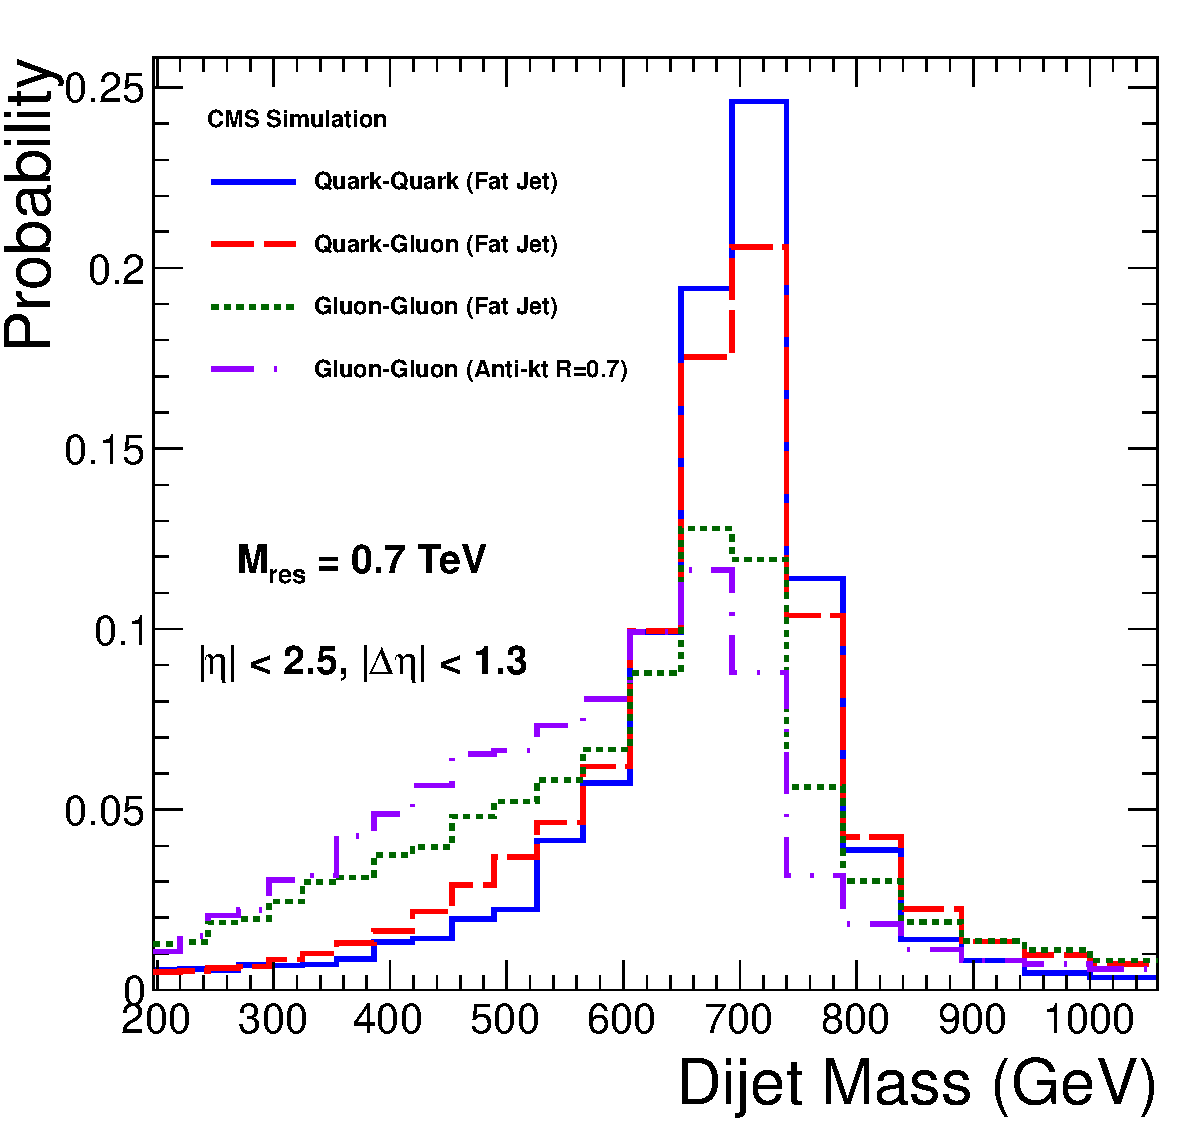
\includegraphics[width=0.45\textwidth]{Figures/shape_700GeV.pdf}
       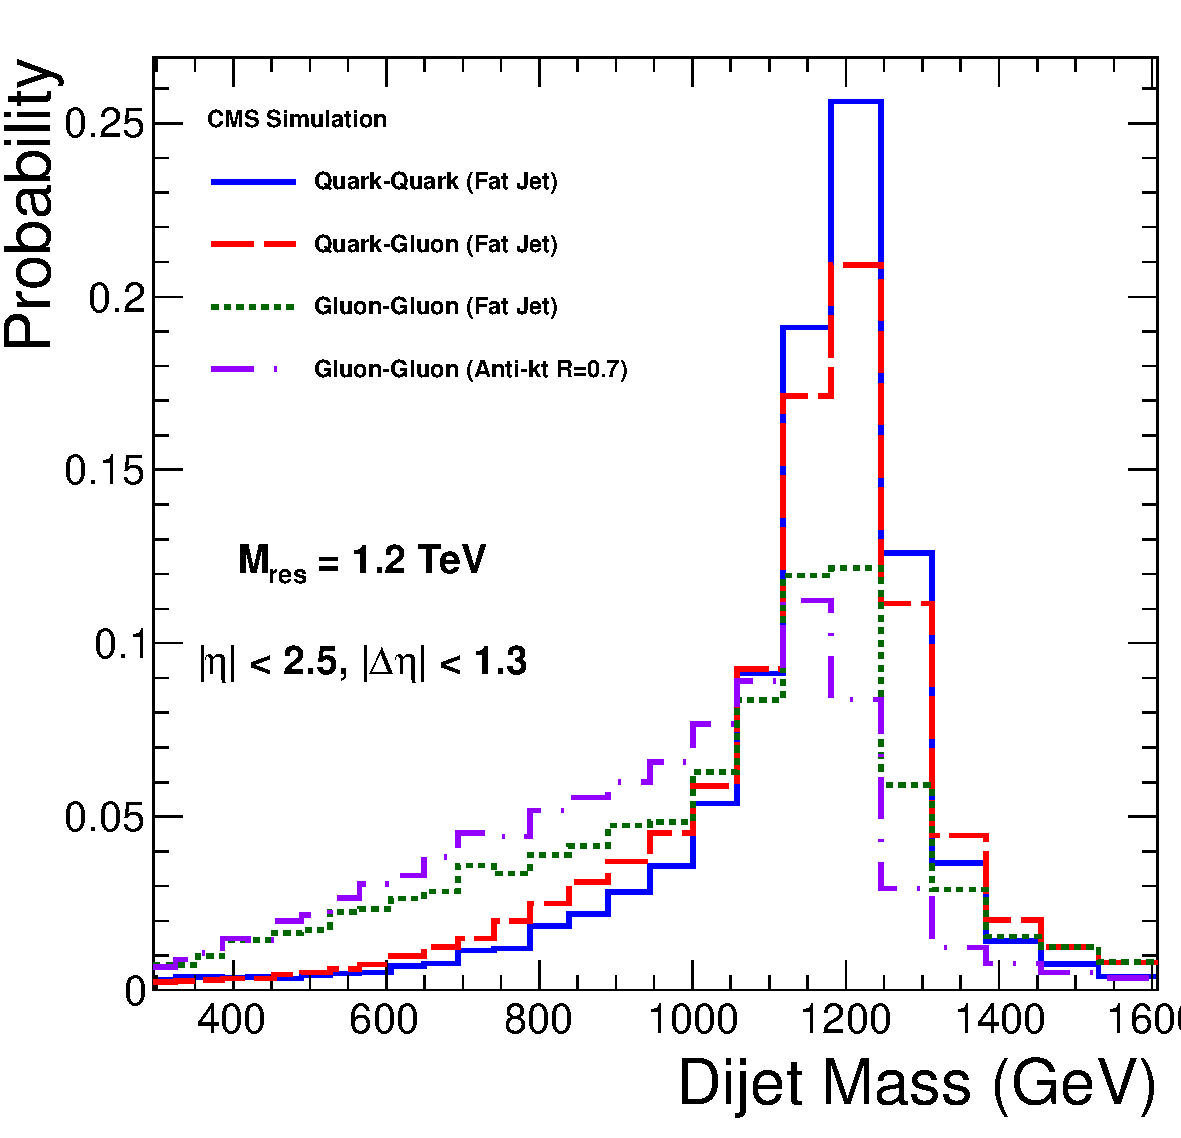
\includegraphics[width=0.45\textwidth]{Figures/shape_1200GeV.pdf}
       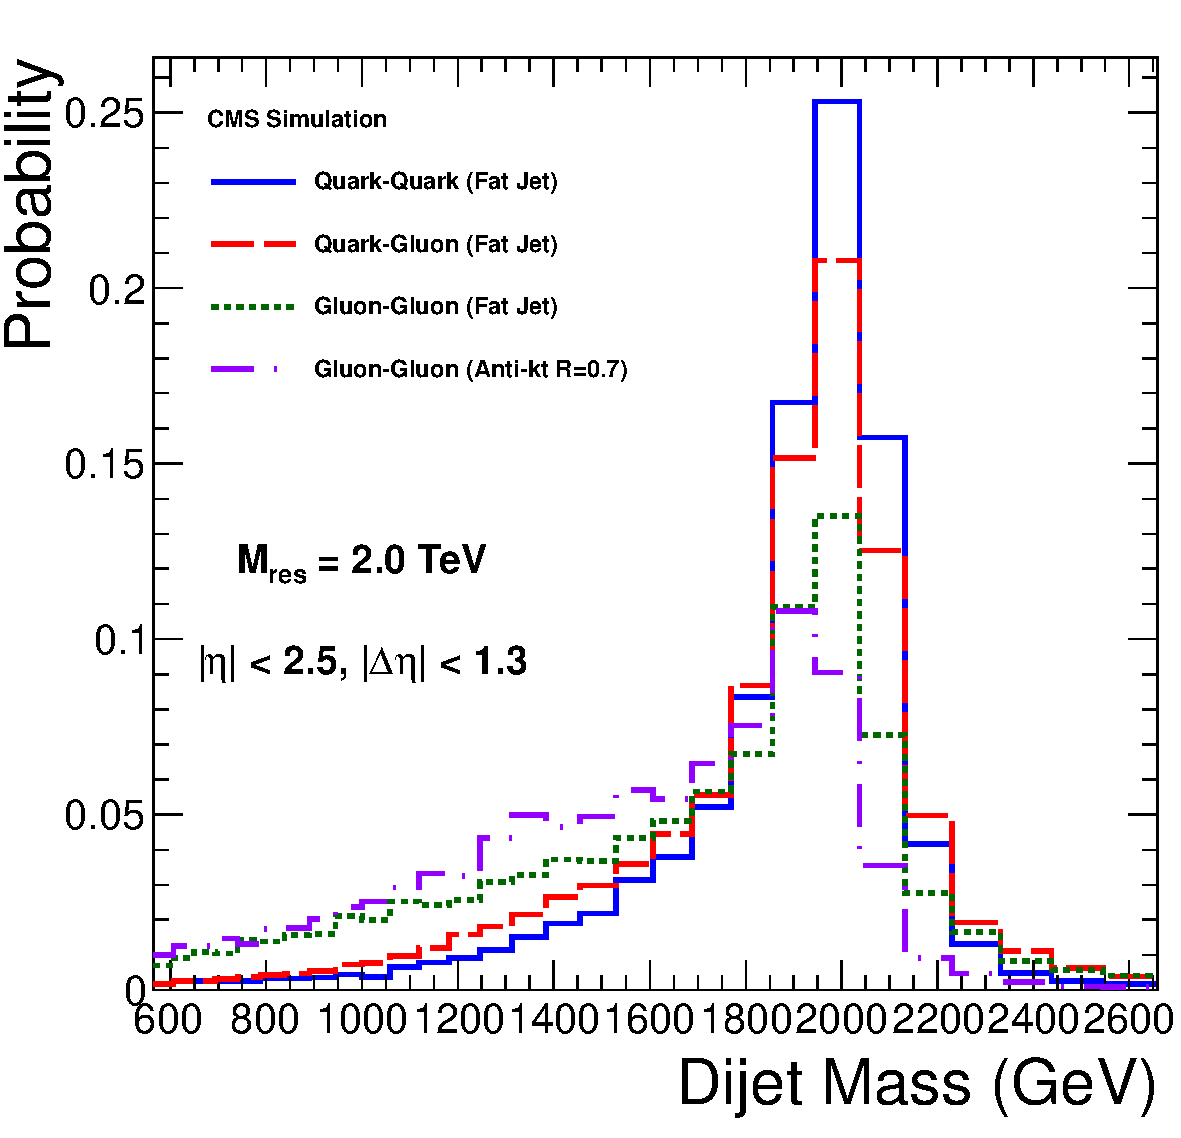
\includegraphics[width=0.45\textwidth]{Figures/shape_2000GeV.pdf}
        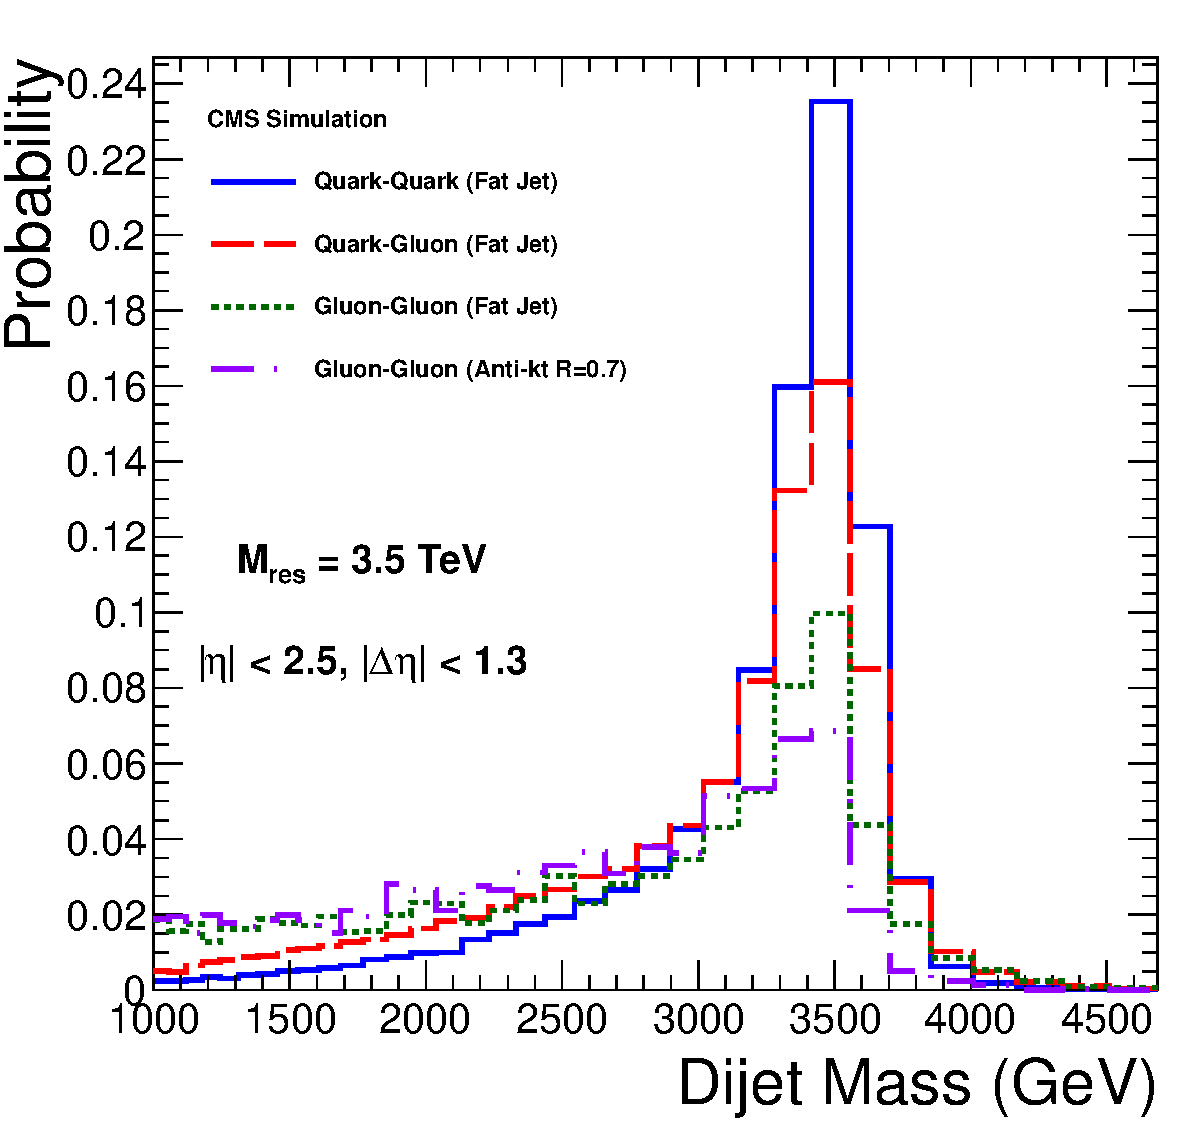
\includegraphics[width=0.45\textwidth]{Figures/shape_3500GeV.pdf}
    \caption{Dijet mass distribution for $q\bar{q}$ $(qq)$, $qg$ and $gg$ resonances at 
    $0.7$, $1.2$, $2$ and $3.5$ TeV resonance mass.}
    \label{resonance_shape}
  \end{center}
\end{figure}



We search for narrow dijet resonances in general, rather 
than a specific model of dijet resonance production.


We require only a model of the resonance line shape. We will only 
consider narrow resonances in this analysis, for which the
natural resonance width is negligible compared to the CMS dijet mass 
resolution, so that the natural width does not affect the resonance shape.
The type of parton pairs in the resonance decay ($qq$, $qg$, or $gg$)
does affect the resonance shape.  To obtain generic shapes for these three
types of parton pairings, the process of $qg\rightarrow q*\rightarrow qg$, 
$q\bar{q} \rightarrow G\rightarrow q\bar{q}$ and 
$gg \rightarrow G\rightarrow gg$ were produced using 
PYTHIA+CMS Spring10 simulation at five different masses of $0.5$, $0.7$, 
$1.2$, $2$ and $3.5$ $TeV$. In Fig.~\ref{resonance_shape} we present four of
these five resonance shapes.



  The source of the shape differences among $qq$, $qg$ and $gg$ resonances 
has been studied previously~\cite{CMS_AN_2009-145}.
The measured width of dijet resonances increases with the number of gluons in the 
final state, primarily
because gluons emit more radiation than quarks.  The peak value of dijet mass of
the resonance decreases with the number of final state gluons, primarily due 
to smaller response of the CMS detector to gluon jets than to quark jets. 
The low mass tail of the resonance shape comes primarily from final state 
radiation. A small high mass tail comes from initial state radiation. 
These resonance shapes are approximately valid for any model of resonance 
involving these pairs of partons, assuming the model's natural half-width 
($\Gamma / 2$) is small compared to the dijet mass resolution.  In 
Fig~\ref{resolution} we present an estimate of the resolution of the Gaussian 
core of the dijet mass response distribution from fits to the peak in an 
interval between $-0.5\sigma$ and $1.5\sigma$.  


\begin{figure}[hbt]
  \begin{center}
     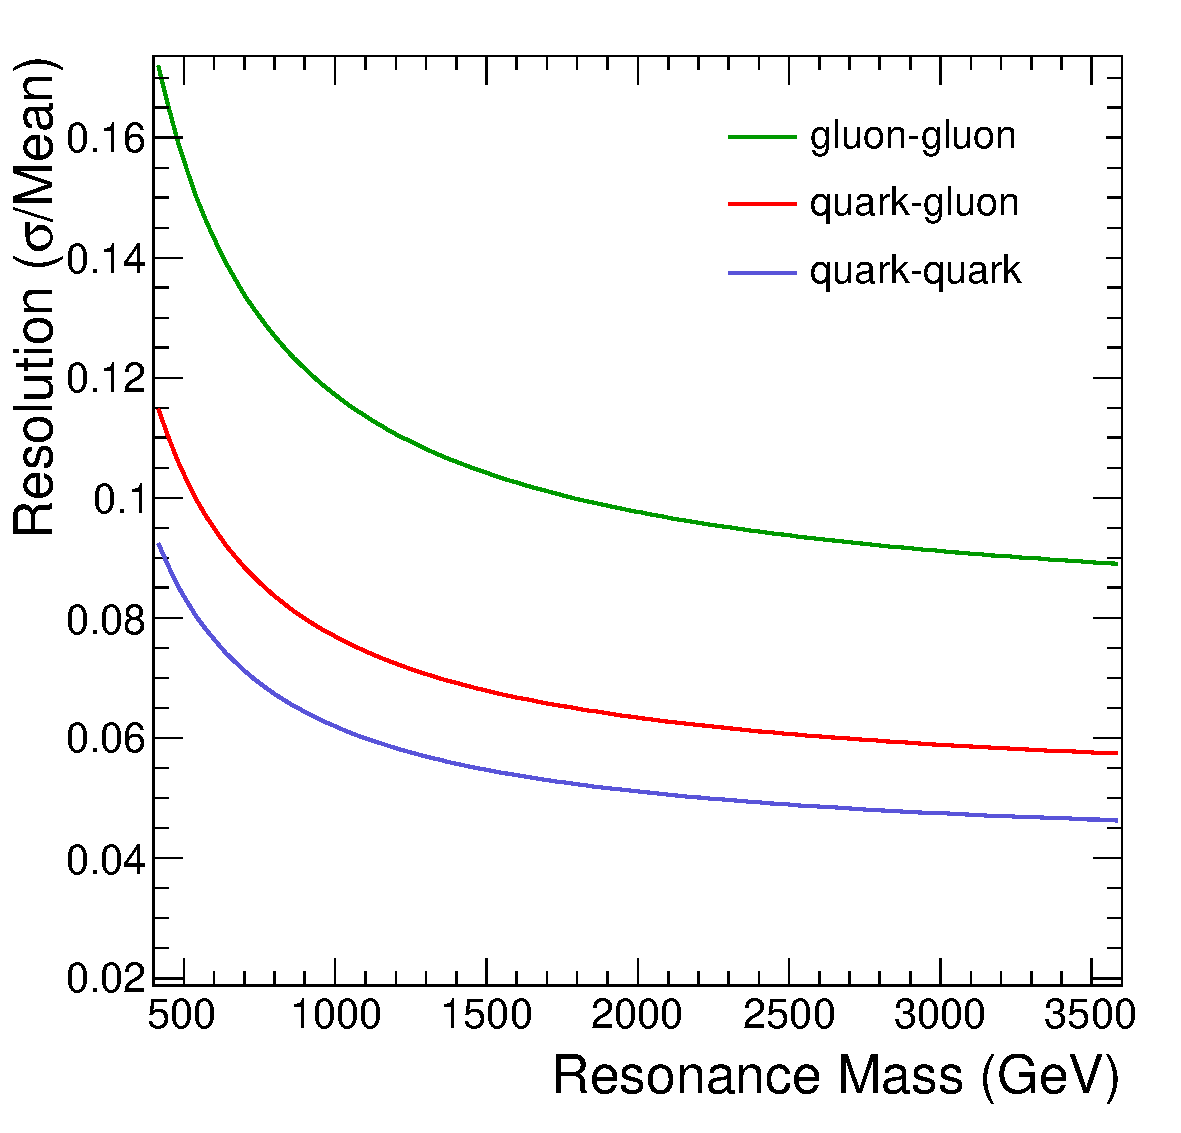
\includegraphics[width=\textwidth]{Figures/Comp_resolution_Color.pdf}
     \caption{The fractional width of the Gaussian core of the response distribution 
     as a function of resonance mass from CMS detector simulations of 
      $qq$, $qg$ and $gg$ dijet resonances.  }
    \label{resolution}
  \end{center}
\end{figure}

Fig.~\ref{shape} shows the simulated signal of excited quarks.
The resonance shape at resonance masses of $M=0.5$,$0.7$, $1.2$, $2.0$ and $3.5$
TeV were obtained from simulation.
We obtain the resonance shapes at intermediate masses via an 
interpolation technique~\cite{CMS_AN_2009-070}. For example the $1.5$ TeV
shape shown in Fig.~\ref{shape} comes from interpolation. The interpolation 
technique
has been checked by doing a wider interpolating between $M=0.7$ and $2.0$ TeV to get the $1.2$ TeV resonance
and comparing that with the actual simulation, and the shapes were the same. 
We use the resonance shapes from our interpolation technique to calculate the cross 
section upper limit at any resonance mass.

\begin{figure}[hbt]
  \begin{center}
     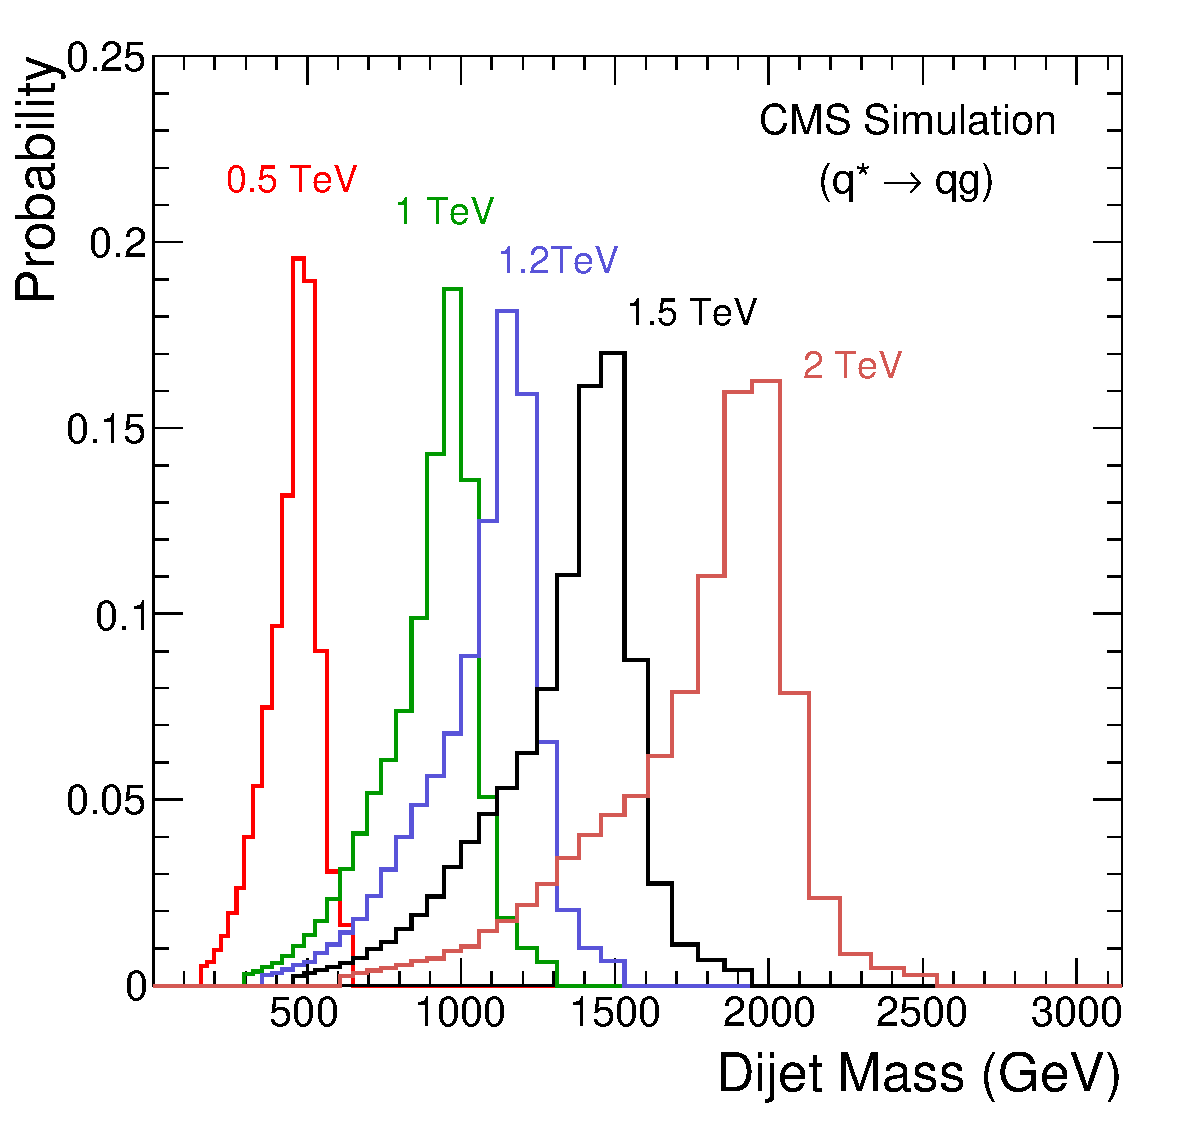
\includegraphics[width=\textwidth]{Figures/Shapes_qg.pdf}
     \caption{$qg$ resonance shapes at various resonance masses coming
     from excited quark simulation at resonance masses in TeV of 
     $0.5$ (red), $0.7$ (green), $1.2$ (blue), $2.0$ (red) and $3.5$ (not shown) and interpolation
     at the example mass of $1.5$ TeV (black).}
    \label{shape}
  \end{center}
\end{figure}

Fig.~\ref{signal_calo} shows the differential 
cross section of excited quark signals as a function of dijet mass 
superimposed on the plot of the dijet mass data with background fit. 
Fig.~\ref{signal_calo} also shows the 
differential cross section of string resonance signals. We model the
string resonance line shape using the excited quark shape since 
string resonances decay predominantly to a
quark and a gluon (see appendix~\ref{appString}) like the excited 
quark. Fig.~\ref{signal_calo} demonstrates that the expected string 
resonance cross section is large, much greater than our measured data.
%The fractional difference between the data and the smooth
%background fit is compared to 
%simulated excited quark resonance signals in Fig.~\ref{fract_signal}, and
%to string resonance signals in Fig.~\ref{fract_signal_string}.  Note 
%the vertical scales are different in Fig.~\ref{fract_signal} and 
%Fig.~\ref{fract_signal_string}.  
In Fig.~\ref{DataOverFit_calo} we show the ratio
between the data and the fit compared to simulated signals for both excited
quarks and string resonances.

\begin{figure}[hbt]
  \begin{center}
     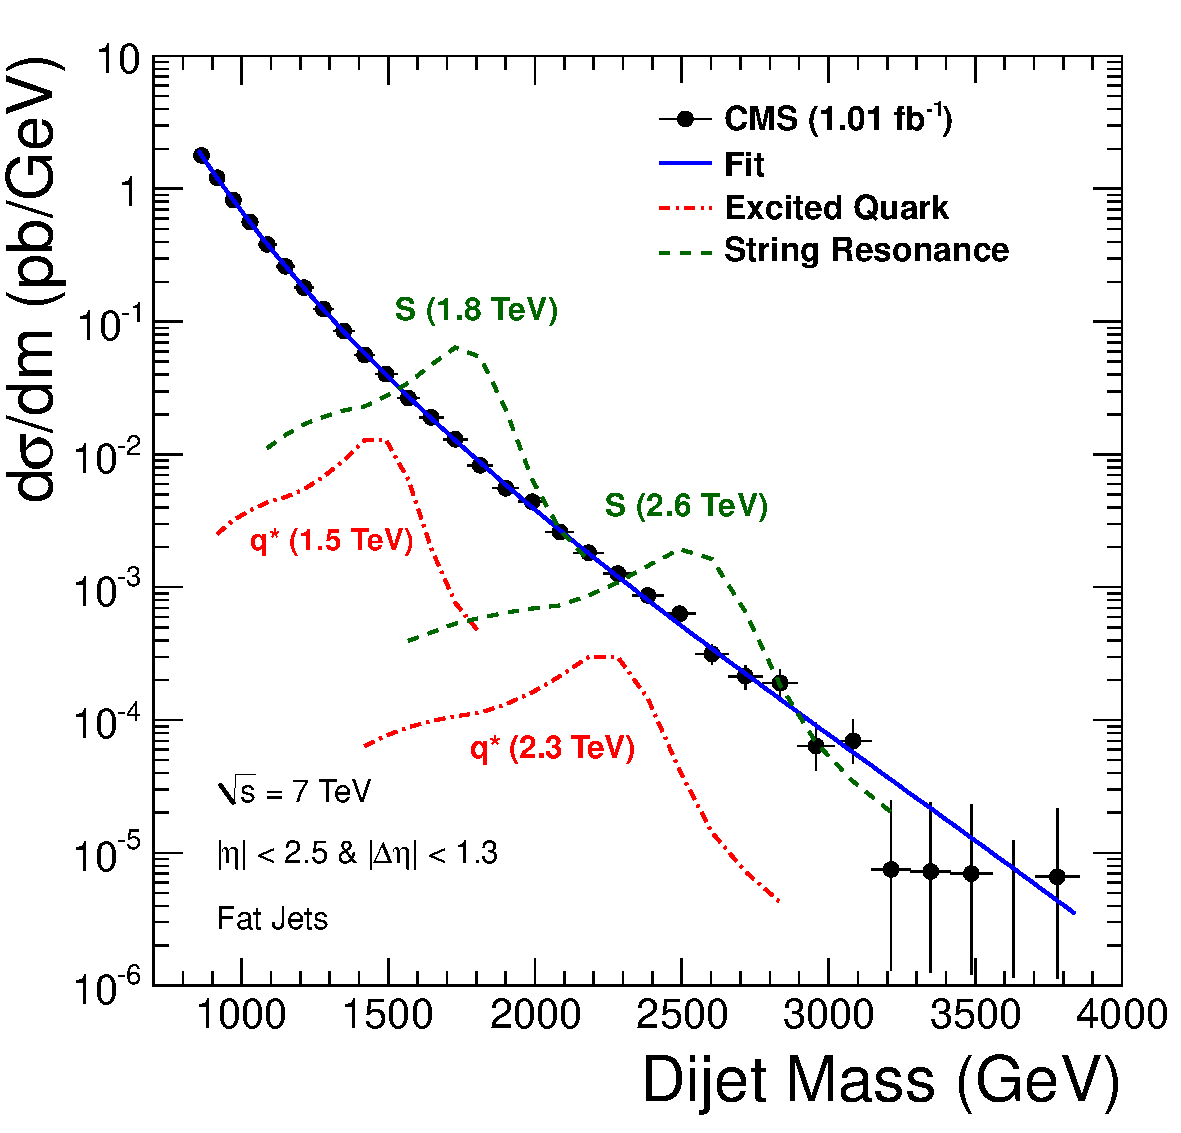
\includegraphics[width=\textwidth]{Figures/DijetMass_withSignal_fat.pdf}
     \caption{The dijet mass distribution for fat jets(points) compared to a smooth
     background fit (blue solid curve) and to a simulation of
     excited quarks (red dot-dashed curves) and string resonances (green dashed
     curves) in the CMS 
     detector.}
    \label{signal_fat}
  \end{center}
\end{figure}

\begin{figure}[hbt]
  \begin{center}
     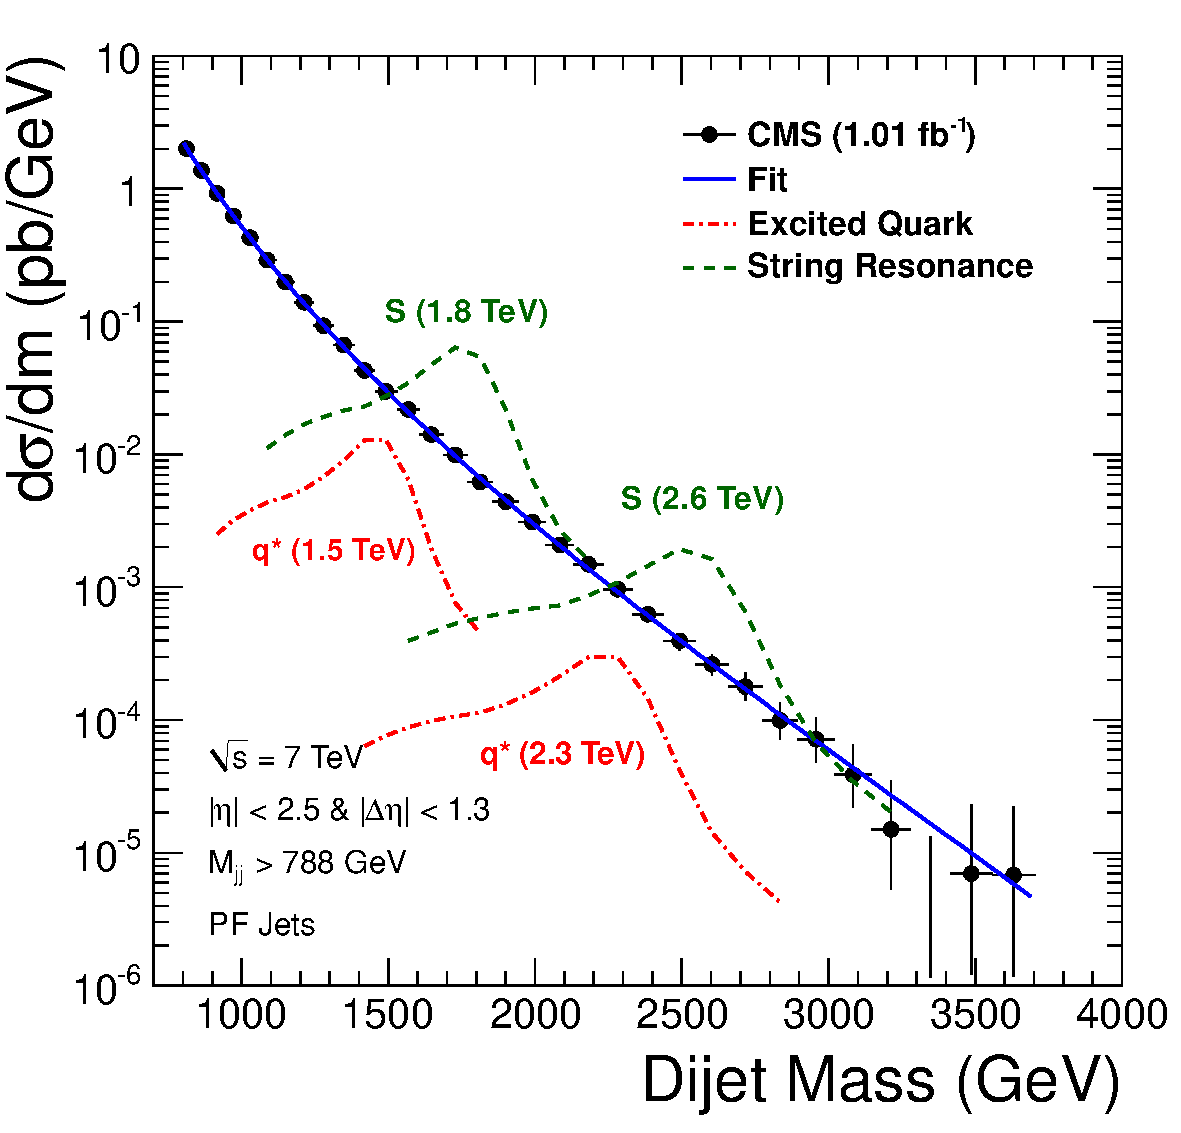
\includegraphics[width=\textwidth]{Figures/DijetMass_withSignal_pf.pdf}
     \caption{The dijet mass distribution for pf jets(points) compared to a smooth
     background fit (blue solid curve) and to a simulation of
     excited quarks (red dot-dashed curves) and string resonances (green dashed
     curves) in the CMS 
     detector.}
    \label{signal_pf}
  \end{center}
\end{figure}

\begin{figure}[hbt]
  \begin{center}
     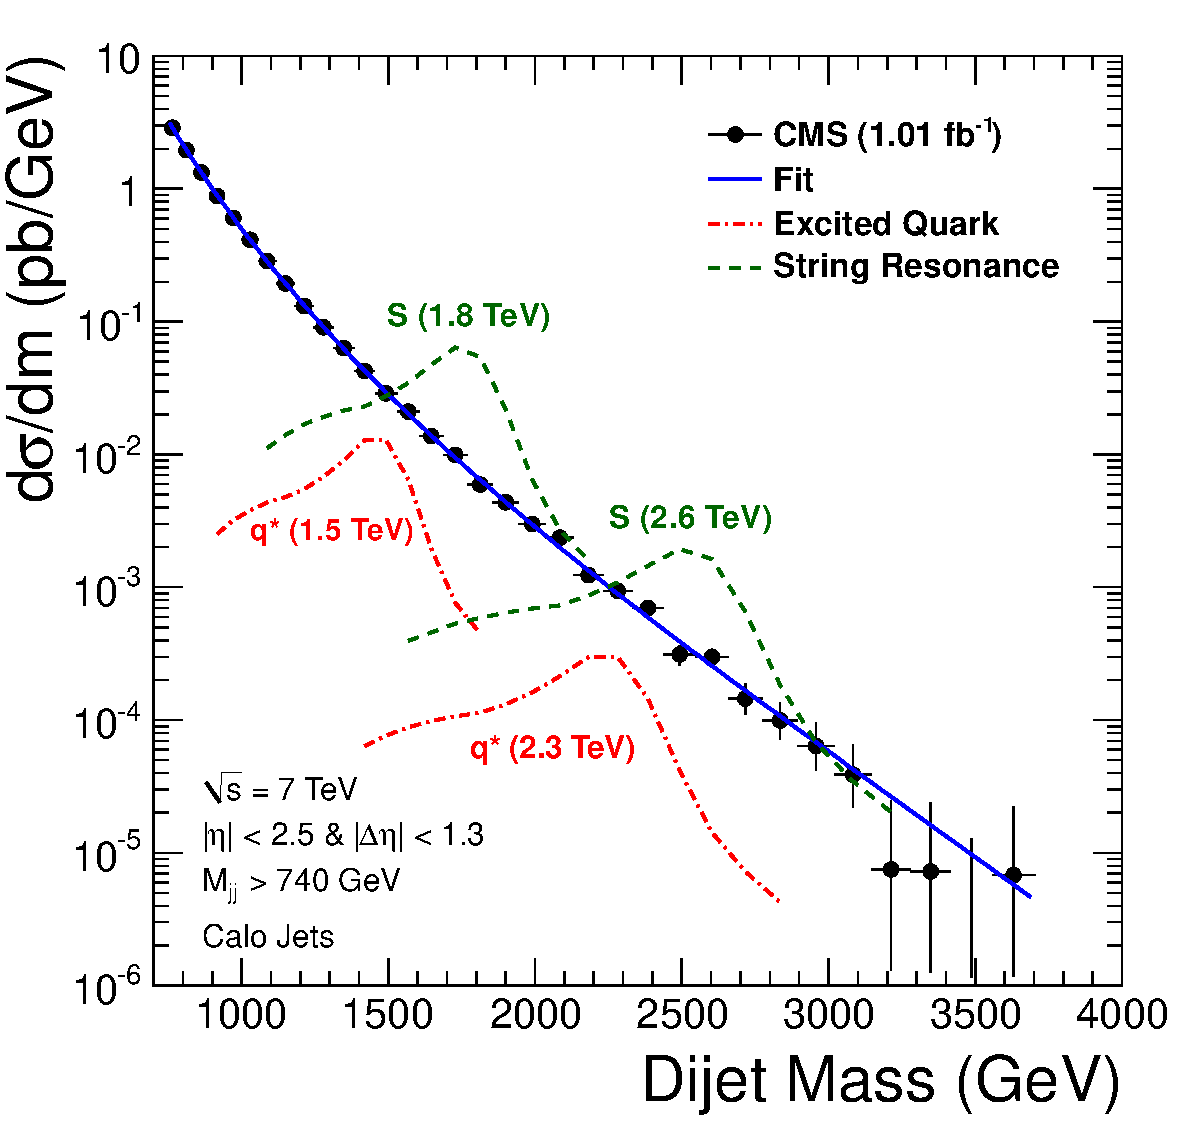
\includegraphics[width=\textwidth]{Figures/DijetMass_withSignal_calo.pdf}
     \caption{The dijet mass distribution for calo jets(points) compared to a smooth
     background fit (blue solid curve) and to a simulation of
     excited quarks (red dot-dashed curves) and string resonances (green dashed
     curves) in the CMS 
     detector.}
    \label{signal_calo}
  \end{center}
\end{figure}

%\begin{figure}[hbt]
%  \begin{center}
%     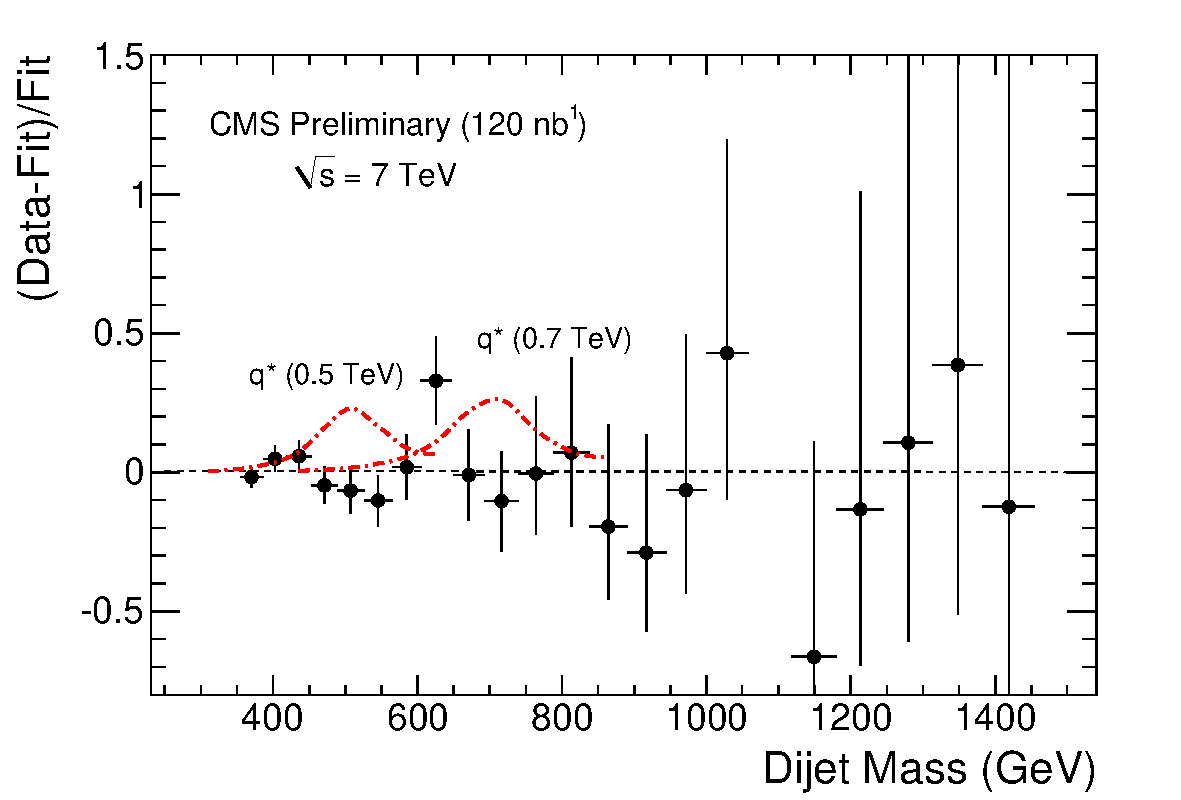
\includegraphics[width=\textwidth]{Figures/Fract_change_withsignal.pdf}
%     \caption{ The fractional difference between the dijet mass distribution (points) and a smooth
%background fit (dashed line) is compared to simulations of excited quark signals in the CMS
%detector (dot-dashed red curves).}
%    \label{fract_signal}
%  \end{center}
%\end{figure}

%\begin{figure}[hbt]
%  \begin{center}
%     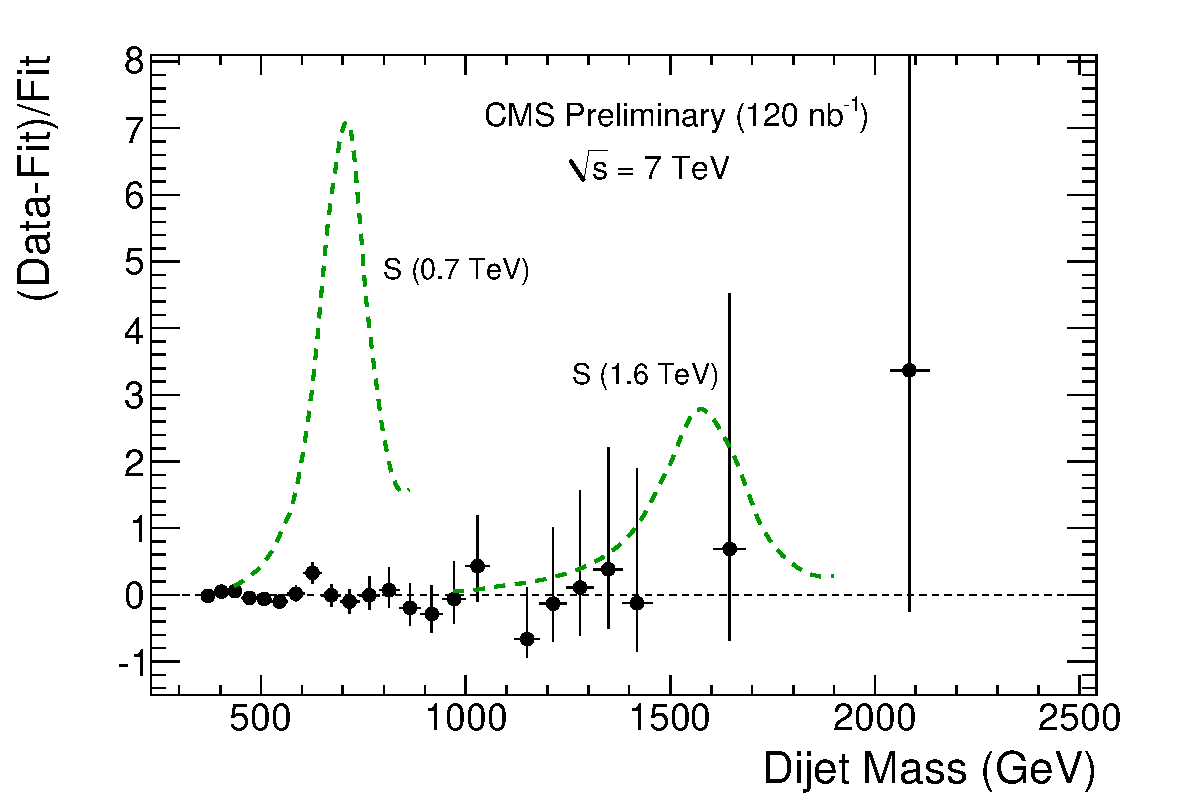
\includegraphics[width=\textwidth]{Figures/Fract_change_withsignal_string.pdf}
%     \caption{ The fractional difference between the dijet mass distribution (points) and a smooth
%background fit (dashed line) is compared to a simulation of a string resonance signal in the CMS
%detector (dashed green curve).}
%    \label{fract_signal_string}
%  \end{center}
%\end{figure}

\begin{figure}[hbt]
  \begin{center}
     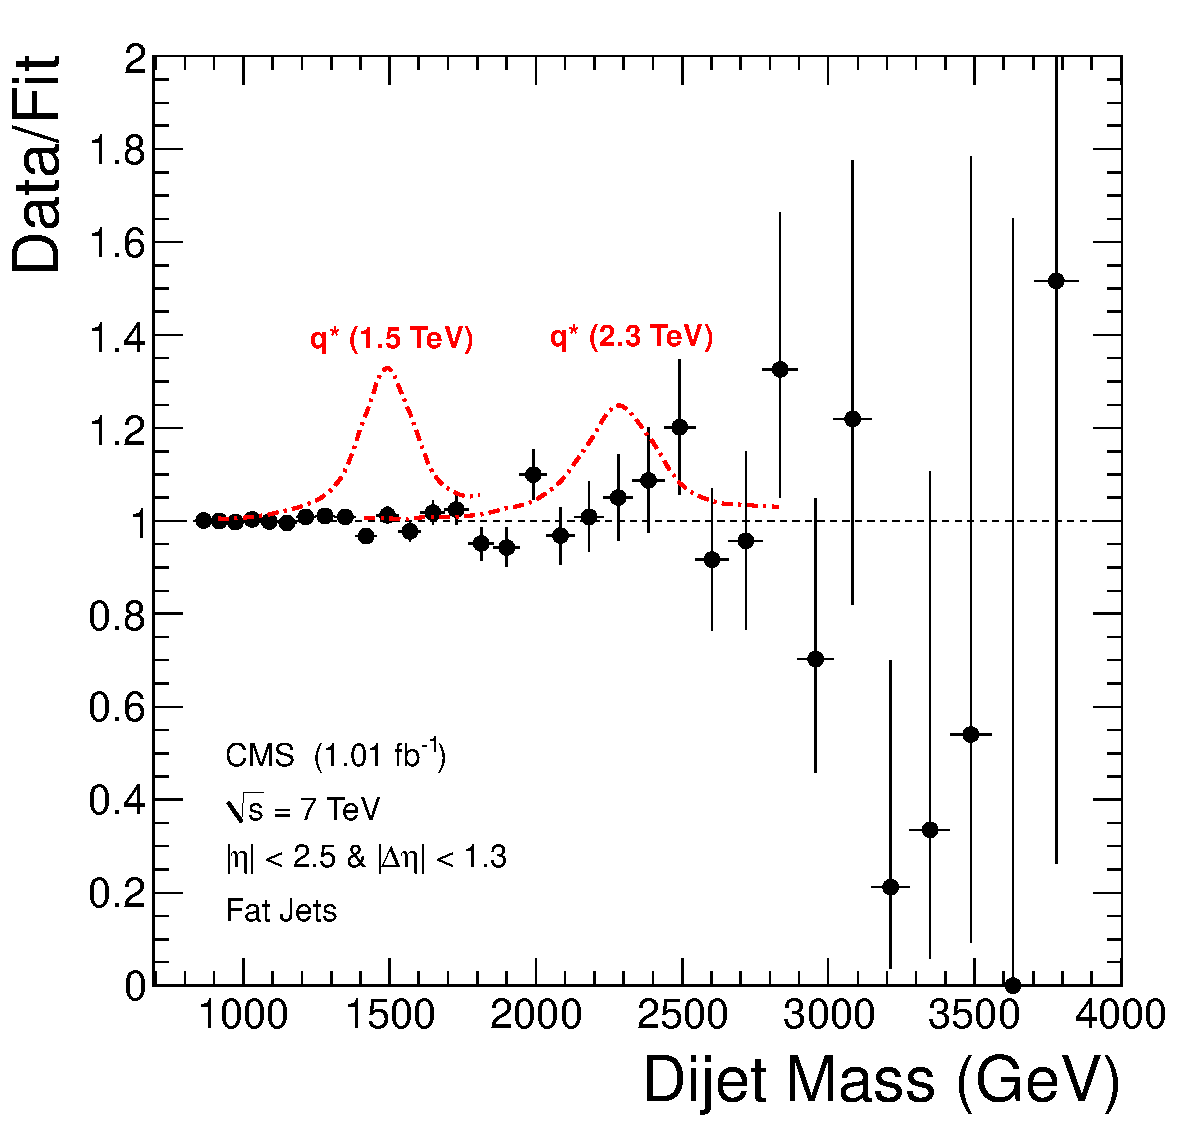
\includegraphics[width=\textwidth]{Figures/data_over_fit_fat.pdf}
     \caption{ The ratio between the dijet mass distribution (points) and a smooth
background fit (dashed line) for fat jets is compared to a CMS detector simulation of an excited quark signal (dashed red curve).}
    \label{DataOverFit_fat}
  \end{center}
\end{figure}

\begin{figure}[hbt]
  \begin{center}
     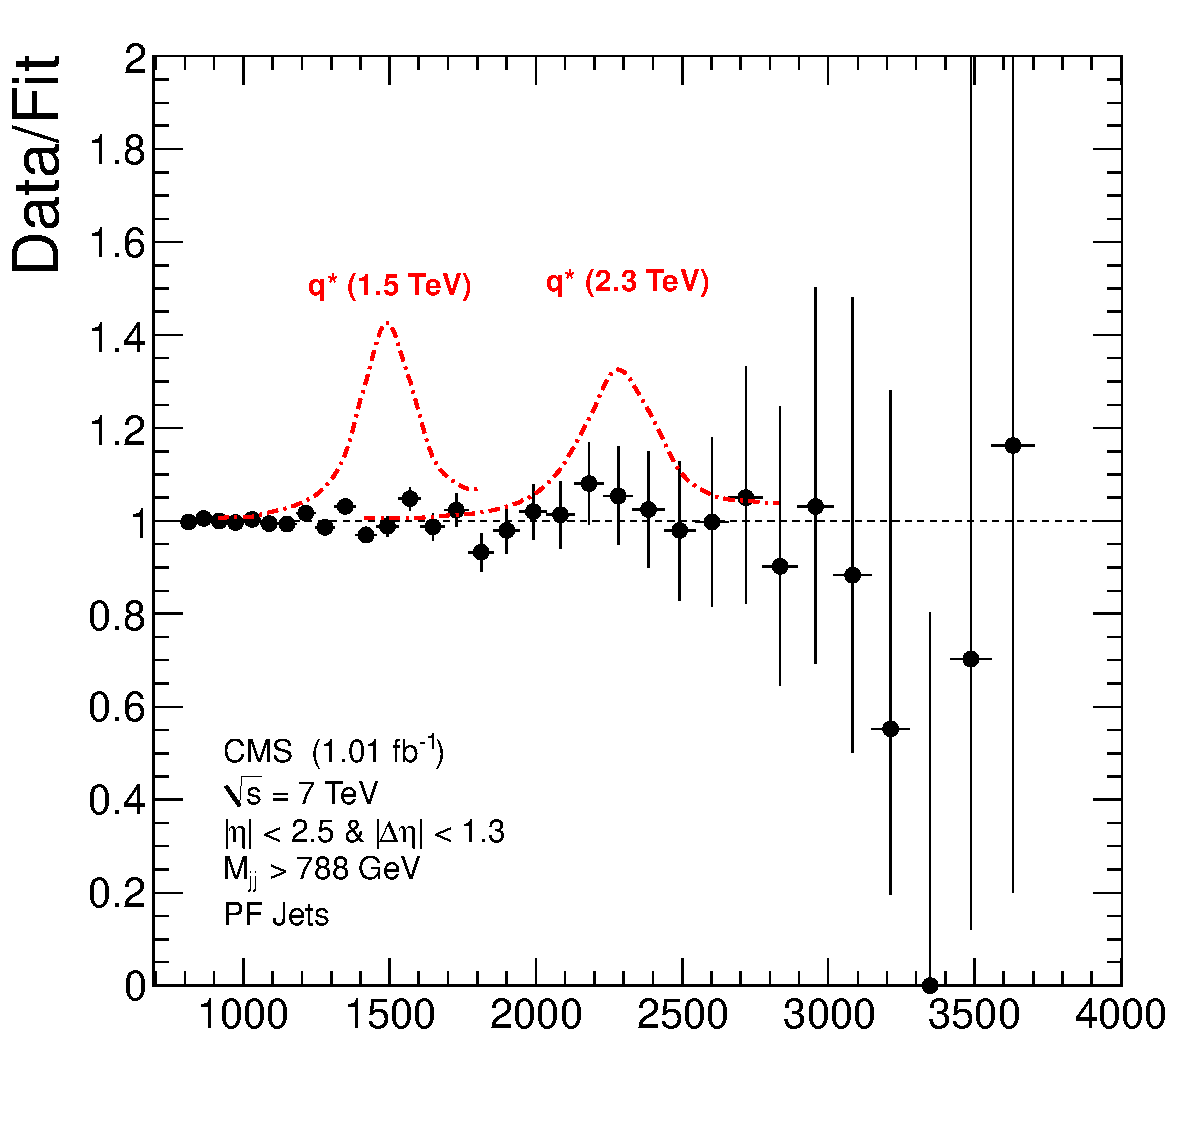
\includegraphics[width=\textwidth]{Figures/data_over_fit_pf.pdf}
     \caption{ The ratio between the dijet mass distribution (points) and a smooth
background fit (dashed line) for pf jets is compared to a CMS detector simulation of an excited quark signal (dashed red curve).}
    \label{DataOverFit_pf}
  \end{center}
\end{figure}

\begin{figure}[hbt]
  \begin{center}
     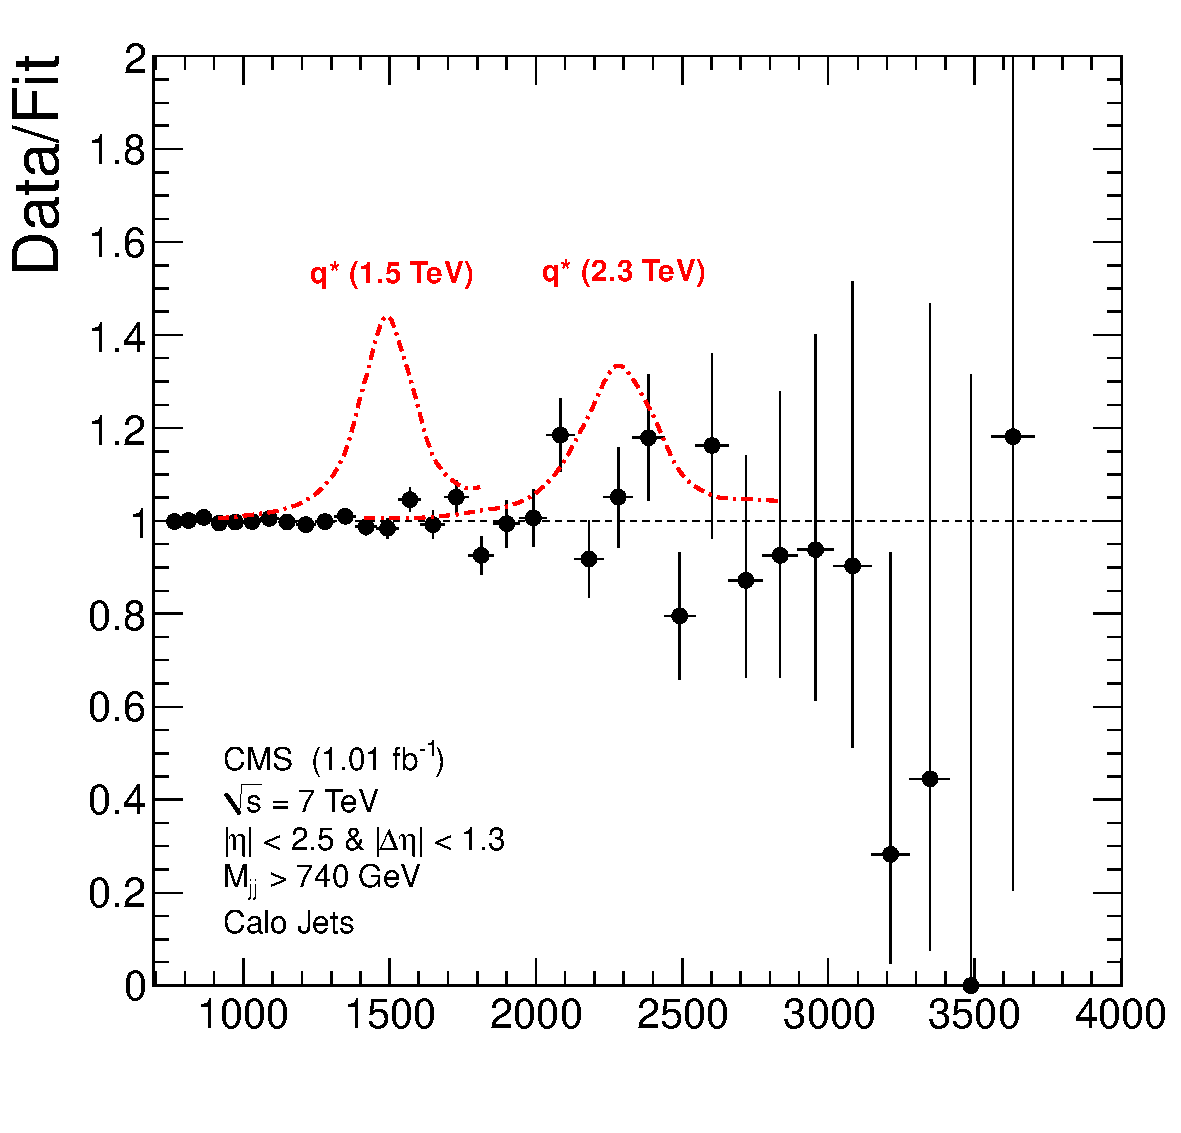
\includegraphics[width=\textwidth]{Figures/data_over_fit_calo.pdf}
     \caption{ The ratio between the dijet mass distribution (points) and a smooth
background fit (dashed line) for calo jetsis compared to a CMS detector simulation of an excited quark signal (dashed red curve).}
    \label{DataOverFit_calo}
  \end{center}
\end{figure}

\clearpage

\subsection {Setting Cross Section Upper Limits}

For setting upper limits on dijet resonance cross section, before accounting for systematic uncertainties,
we begin with a Bayesian formalism with uniform prior for the cross section.
The binned likelihood, $L$, as a function of a constant $\alpha$ can be written as:
\\
\begin{equation}
L = \prod_{i} \frac{\mu_{i}^{n_{i}}e^{-\mu_{i}}}{n_{i}!}
\end{equation}
\\
where
\\
\begin{equation}
\mu_{i} = \alpha N_{i}(S) + N_{i}(B),
\end{equation}
\\
$n_{i}$ is the measured number of events in the $i^{th}$ dijet mass bin, $N_{i}(S)$ is the number of events from the signal in the $i^{th}$ dijet mass bin,
$\alpha$ is a constant to scaling the signal amplitude, and $N_{i}(B)$ is the number of expected events from background in the $i^{th}$ dijet mass bin.
We consider that the QCD background is fixed by the best $Signal+QCD$ fit to the data points and it gives the expected number of background event in the $i^{th}$
dijet mass bin, $N_{i}(B)$. The number of signal events in the $i^{th}$ dijet mass bin, $N_{i}(S)$, comes from an interpolation technique.
The signal range is chosen to be from $0.3\cdot M_{Res}$ to $1.3\cdot M_{Res}$, an interval which contains nearly all the resonance
line shape.
We assume a flat prior in $\alpha$, which is the same as a flat prior in the resonance cross section.  With this assumption
the likelihood normalized to unity is equivalent to a posterior probability density, and can be used to set limits.  
We calculate the posterior probability density as a function of signal cross section for resonances with 
mass from $0.6$ TeV to $3.3$ TeV in $0.1$ TeV steps.  Example likelihoods are shown in the appendix of  
AN-2010/108-v14 dated October 20, 2010 for the 3 pb$^{-1}$ dataset.
The 95\% confidence level upper limit $\sigma_{95}$ is calculated from the posterior probability density $P_{POST}$ as follows:

\begin{equation}
\frac{\int_{0}^{\sigma_{95}} P_{POST}(\sigma)d\sigma}{\int_{0}^{\infty} P_{POST}(\sigma)d\sigma} = 0.95
\end{equation}

%In Fig.~\ref{Likelihood}, Likelihood distribution at $0.7$ GeV resonance masses for $qg$ resonances are illustrated. The likelihood distributions 
%for resonance mass from $0.5$ TeV to $1.5$ TeV in $0.1$ TeV step can be seen in Appendix X.
%
%\begin{figure}[!ht]
%  \begin{center}
%    \includegraphics[width=0.55\textwidth]{Figures/Likelihood_700GeV.pdf}
%    \caption{Likelihood Distribution with statistical error only.}
%    \label{Likelihood}
%  \end{center}
%\end{figure}


We present the 95\% CL upper limit on dijet resonance cross section in 
Fig.~\ref{Limit_statonly_calo} including only statistical uncertainties. 
Quark-quark, quark-gluon, and gluon-gluon 
resonances are shown separately. The limits have small wiggles 
corresponding to structures in the data and the width of the
resonance line shape.  
The limits are also tabulated numerically in table~\ref{tabStatLimit_calo}. 
%At the highest resonance mass shown,
%2.6 TeV, the limits have a value of between 4 and 6 events. This corresponds to 
%the few events observed in the tail of the dijet mass distribution that are 
%still within the resonance line shape.  
%In prior analysis versions, where there were no events 
%at high dijet mass, we have shown explicitly that the limit plateaus at exactly 3 
%events, corresponding to 0 events observed.  


\subsection {Limit Setting with Roostat}

Until the AN-2010/018-v15, we made our own code to set limit based on a Bayesian method
fitting the data in our large variable sized bins with the data assigned to the center of the bin. 
In that method the data point was simply fit by a parameterization.
From now on we use Roostat to impliment the Bayesian method, since it's the official tool for statistics
now at CMS. Roostat is a statistical tool built on top of RooFit. In the new method the parameterization
is a density function which is integrated over the bin used to find the value within the bin. In the new
method the bin size is very fine, 1 GeV. 
%Using old method 
%and new method basically produce almost same result as you see in Fig~\ref{Limit_statonly_old_new}.
%The small difference is due to the differences in the fit when integrating the density over fine
%bins in the new method versus using the bin center in a fit with coarse variable bins in the old method.
%We verified for a previous dataset that when shrinking the coarse bins in the old method the two methods 
%converged towards the same result.
We fit the data after we make the dijet mass histogram from the trigger cut to 5 TeV with bin size
1 GeV in new method. 
%The 838 GeV lower edge of the dijet mass histogram comes from our dijet mass cut for more
%than 99.8\% trigger
%efficiency. 
The 5 TeV upper edge on dijet mass histogram allows us to use data up to that point to calculate
limits safely up to a resonance mass of 4 TeV. Once we get the background fit we follow the process that we descibed in previous section.
%Fig~\ref{Limit_statonly_old_new} shows both the new method using our Bayesian calculator, which has been
%constructed to permit fast and effective integrations necessary to include the systematics later, and also
%the results using the "out of the box" MCMC calculator, which is too slow to include systematics.  The results
%from our calculator agree almost exactly with the MCMC calculator.

%\begin{figure}[!ht]
%  \begin{center}
%    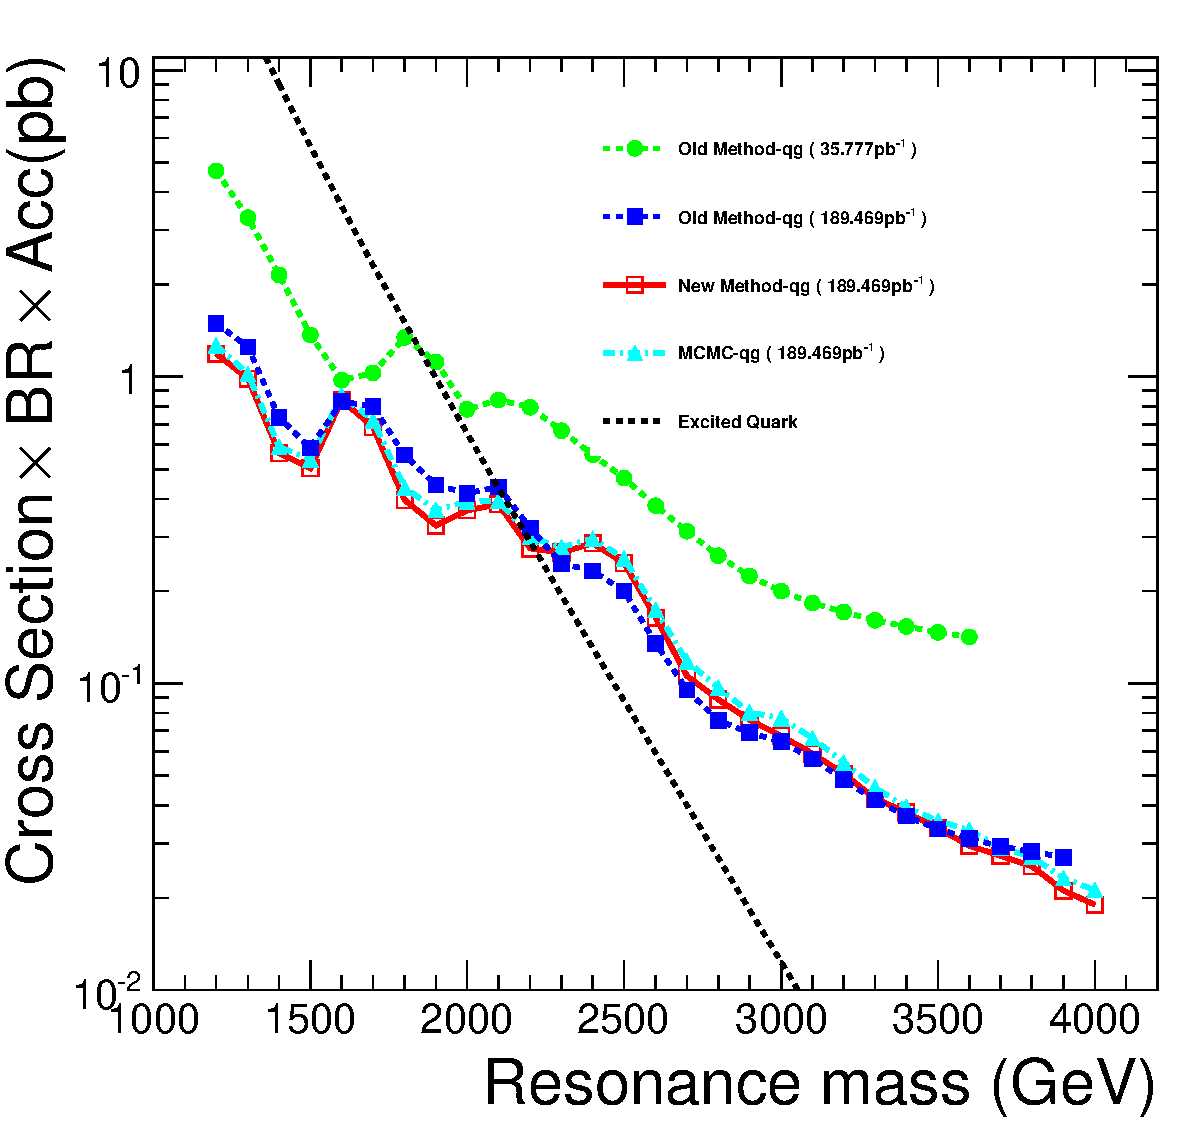
\includegraphics[width=\textwidth]{Figures/stat_limit_compare_old_new.pdf}
%    \caption{Dijet resonance sensitivity with statistical errors only. The 95\% C.L.
%      upper limit on cross section is compared to the cross section for old and new
%      methods. This sensitivity does not contain estimates of the systematic uncertainties.
%      Result from MCMC is also presented.}
%    \label{Limit_statonly_old_new}
%  \end{center}
%\end{figure}

\begin{figure}[!ht]
  \begin{center}
    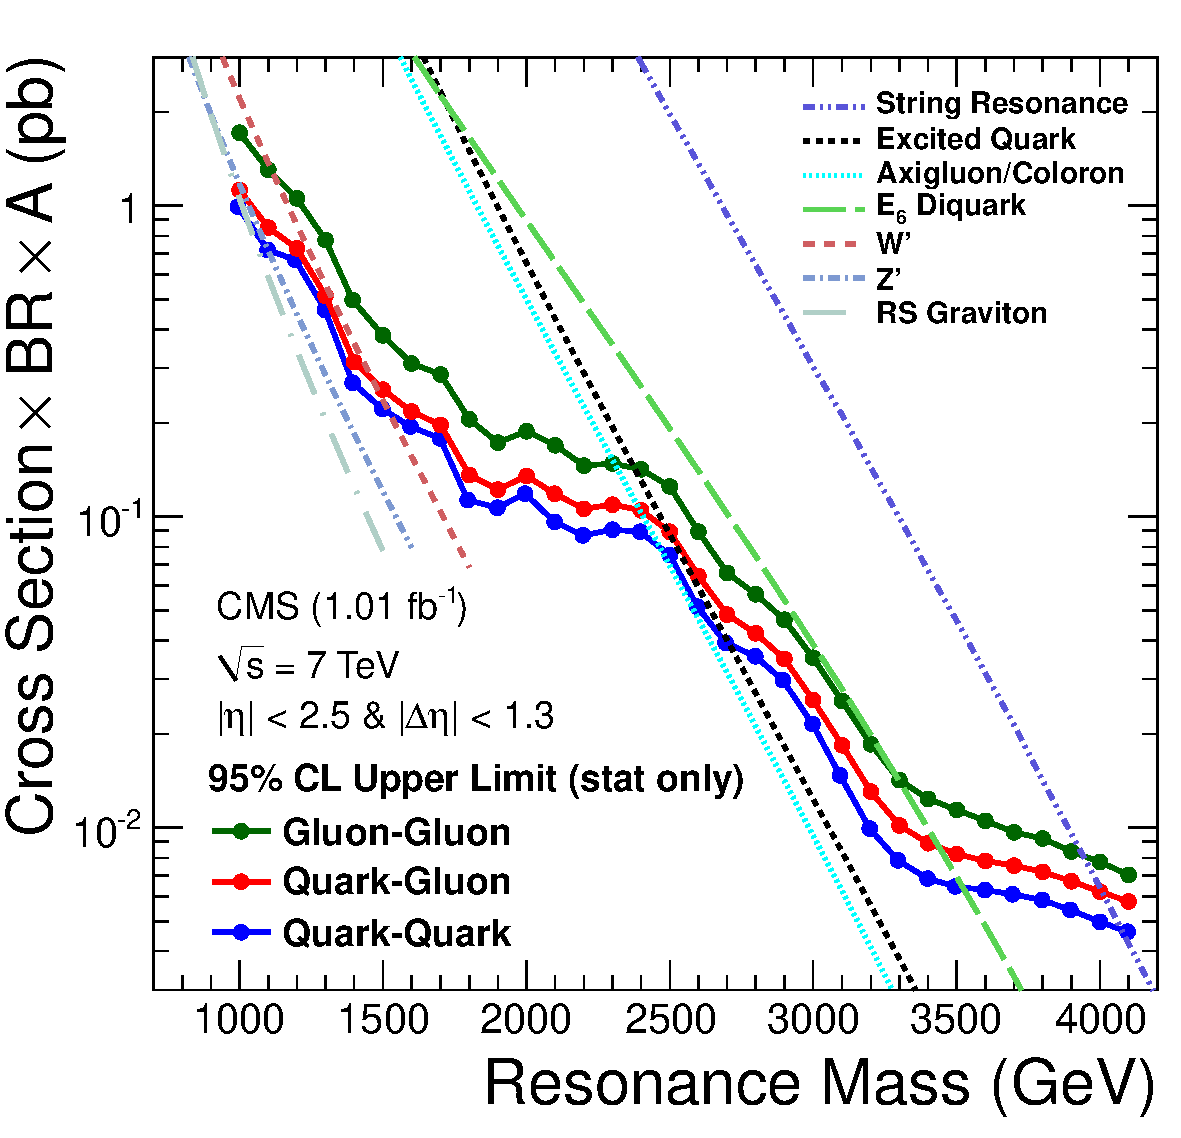
\includegraphics[width=\textwidth]{Figures/c_xs_stat_fat.pdf}
    \caption{Dijet resonance sensitivity with statistical errors only for fat jets. The 95\% C.L. upper limit on cross section 
    is compared to the cross section for various resonance models.
This sensitivity does not contain estimates of the systematic uncertainties.}
    \label{Limit_statonly_fat}
  \end{center}
\end{figure}

\begin{figure}[!ht]
  \begin{center}
    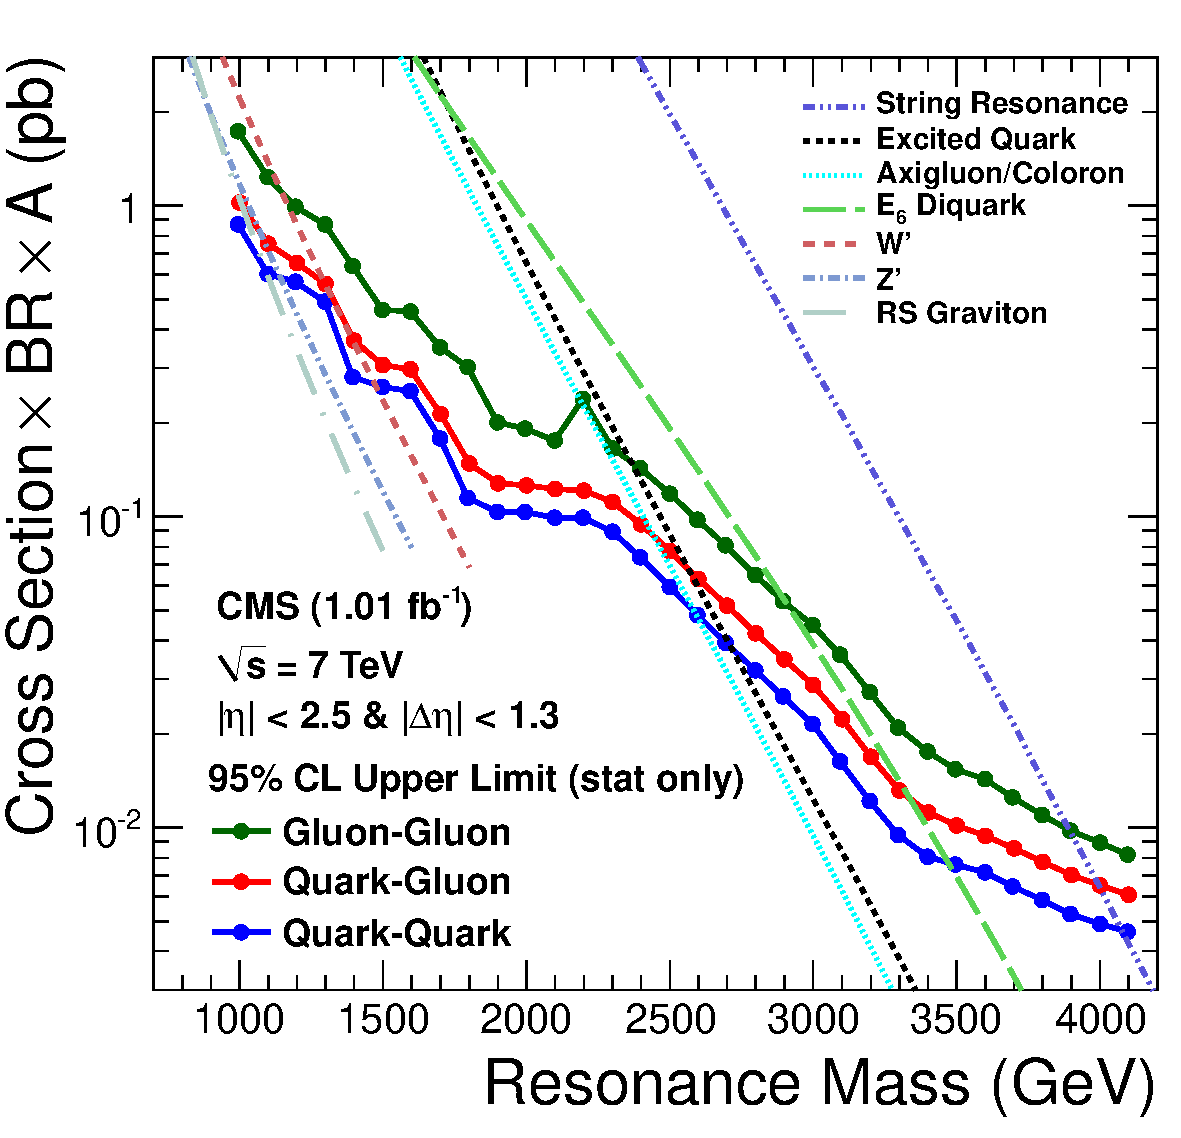
\includegraphics[width=\textwidth]{Figures/c_xs_stat_pf.pdf}
    \caption{Dijet resonance sensitivity with statistical errors only for pf jets. The 95\% C.L. upper limit on cross section 
    is compared to the cross section for various resonance models.
This sensitivity does not contain estimates of the systematic uncertainties.}
    \label{Limit_statonly_pf}
  \end{center}
\end{figure}

\begin{figure}[!ht]
  \begin{center}
    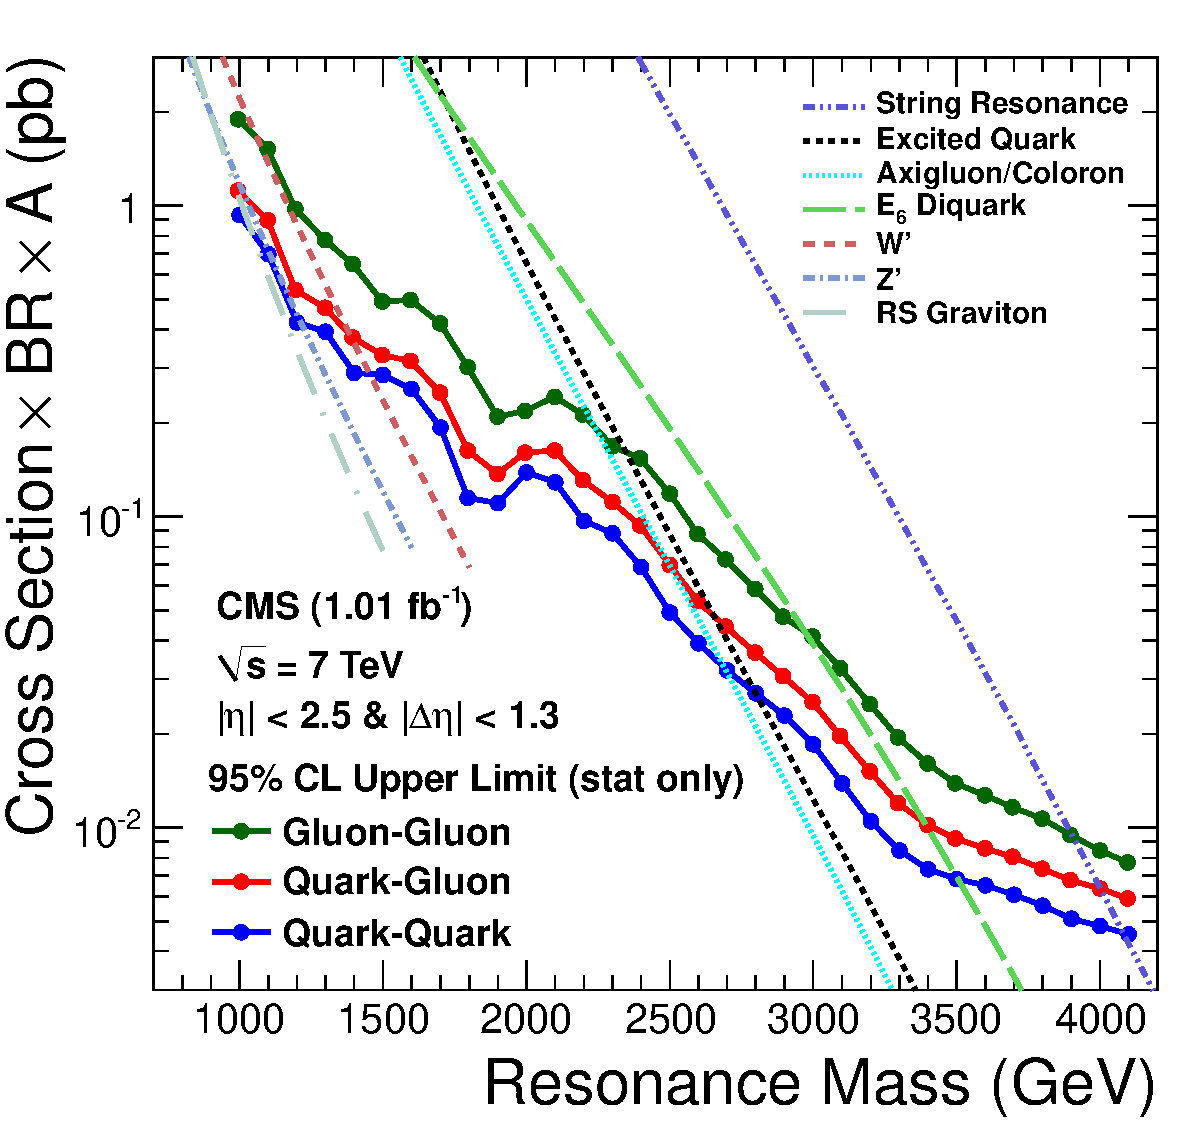
\includegraphics[width=\textwidth]{Figures/c_xs_stat_calo.pdf}
    \caption{Dijet resonance sensitivity with statistical errors only for calo jets. The 95\% C.L. upper limit on cross section 
    is compared to the cross section for various resonance models.
This sensitivity does not contain estimates of the systematic uncertainties.}
    \label{Limit_statonly_calo}
  \end{center}
\end{figure}

%The procedure used in this note dates
%from one used by the CDF collaboration in Tevatron run I~\cite{Abe:1995jz,Abe:1997hm}, which was superseded in CDF run II~\cite{Aaltonen:2008dn} by a
% more fully
%Bayesian treatment of nuisance parameters. The newer CDF method
%(implemented in code by Ken Hatakeyama) gives a cross section upper
%limit which is roughly 10\% better than that in this note, presumably due
%to better treatment of the systematics, as discussed in the next section. 

%We have checked this procedure with independent software written for CDF by one of us (Ken Hatakeyama). 
%The CDF software gives a cross section upper limit that is pretty close, roughly 10\% better (smaller) 
%than ours, and we have not yet understood this small difference. We have also used the CDF software to 
%modify the basic limit setting method that we used, using a profile likelihood (posterior probability density).  
%The profile likelihood allows the background parameters to vary at every signal cross section point in the 
%likelihood, instead of fixing the background at the best $Signal+background$ fit. We note that CDF used the
%profile likelihood method in run 2~\cite{Aaltonen:2008dn}, and used the method of fixing the background at the best $Signal+background$ fit
%in run 1~\cite{Abe:1997hm}.  The resulting change between the two different methods in the limit for our dataset is small, 
%increasing by roughly 10-20\% at low masses and yielding in the end a very
%similar limit to the default machinery we use for limits.  
%More work needs
%to be done to incorporate the systematics into the profile likelihood 
%machinery, and to integrate the smooth operation of that machinery with our 
%personnel, before we can effectively use it to set limits.  We are encouraged 
%by the small difference between the two methods compared to our total 
%systematics described in the next section.

%\begin{figure}[!ht]
%  \begin{center}
%    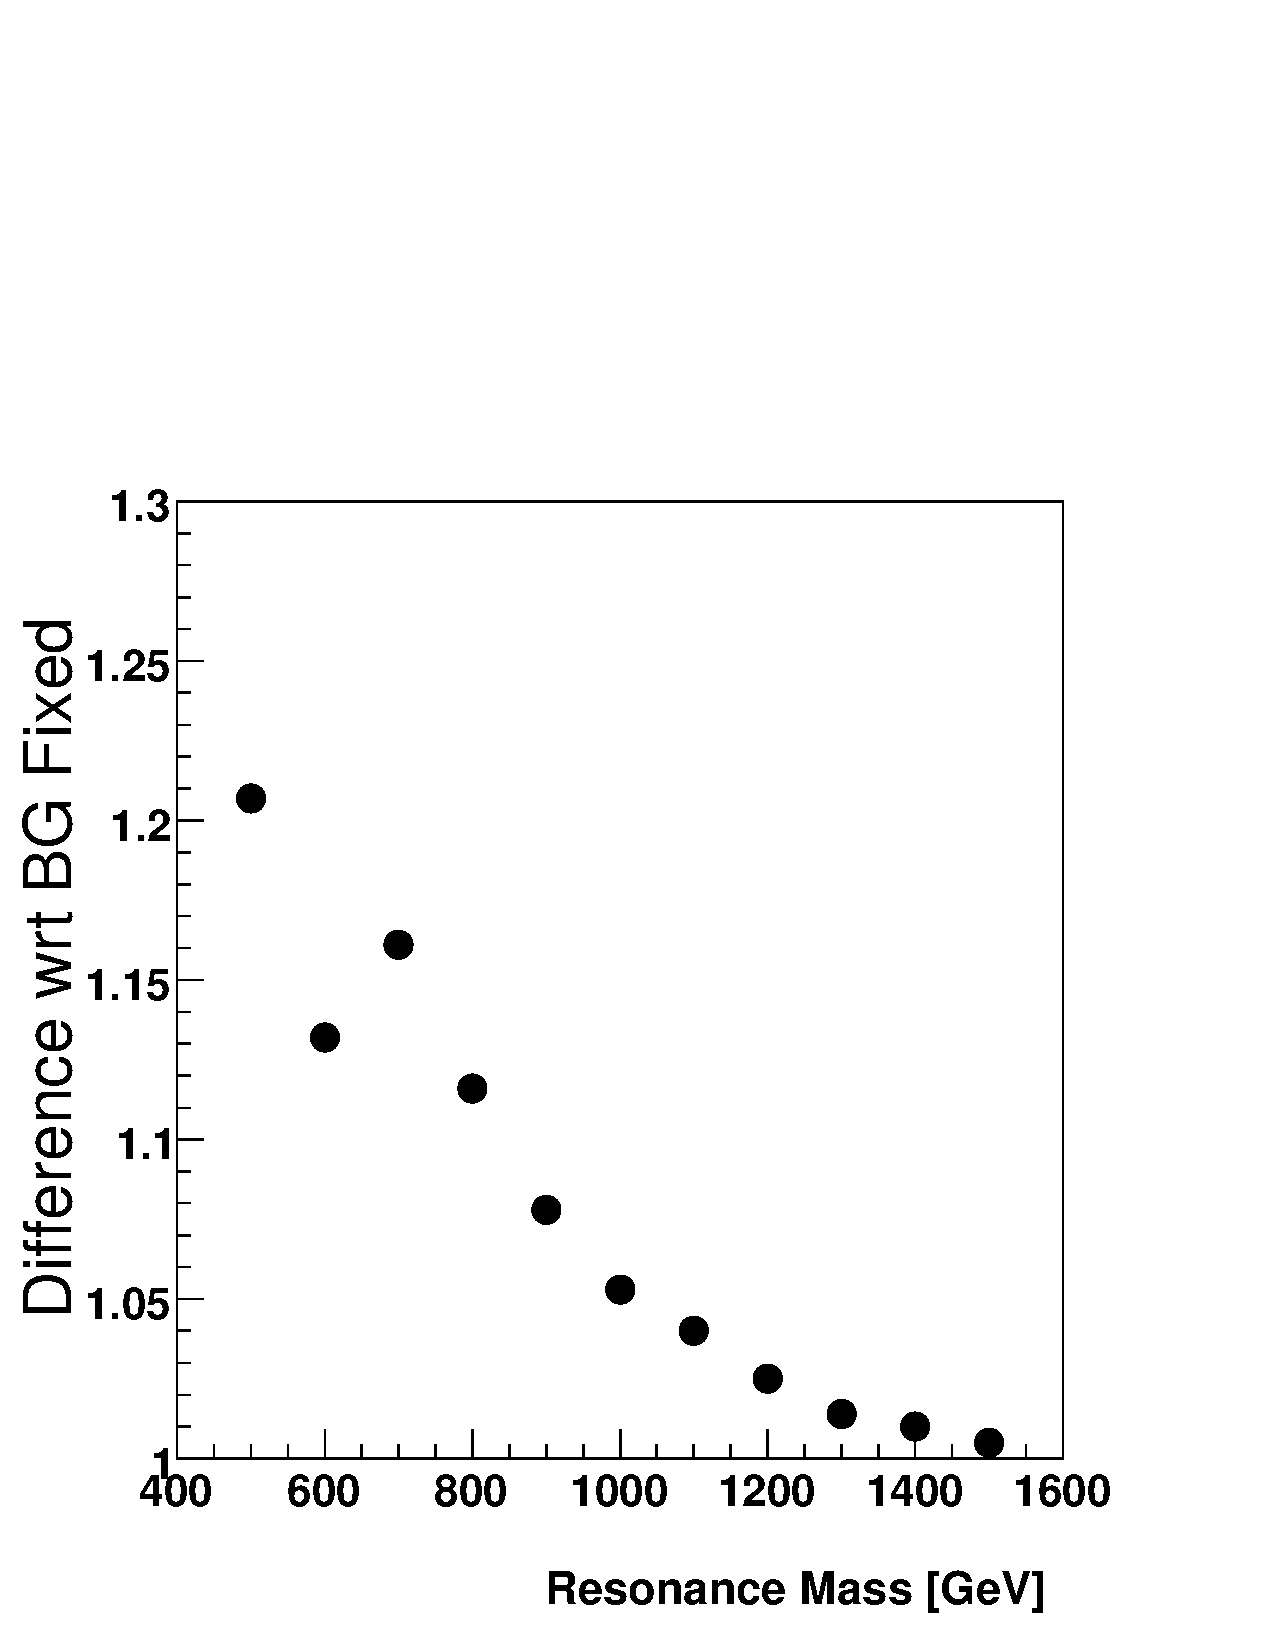
\includegraphics[width=0.7\textwidth]{Figures/DijetMassLimitsProfileLikelihood}
%    \caption{Changes in the 95\% CL upper limits on the $qg$ resonance
%      cross section as a function of resonance masses when the profile
%      likelihood is used, compared to the case in which the background
%      parameters are fixed at the best $Signal+background$ fit. 
%      Analysis done independently with statistics software from CDF (see text).}
%    \label{LimitsProfileLikelihood}
%  \end{center}
%\end{figure}




\begin{table}[htbH]
\centering
\large
\begin{tabular}{|c|c|c|c|}\hline
Mass   &  \multicolumn{3}{c|}{95\% C.L. $\sigma\cdot B$ (pb) Stat. Err. Only}\\
 ($TeV$) & quark-quark       & quark-gluon  & gluon-gluon\\ \hline
1.0 & 0.98117 & 1.12380 & 1.71707 \\
1.1 & 0.71763 & 0.85015 & 1.30642 \\
1.2 & 0.66727 & 0.72977 & 1.05537 \\
1.3 & 0.46010 & 0.51269 & 0.77611 \\
1.4 & 0.26575 & 0.31458 & 0.49823 \\
1.5 & 0.22164 & 0.25654 & 0.38314 \\
1.6 & 0.19445 & 0.21768 & 0.31132 \\
1.7 & 0.17629 & 0.19703 & 0.28691 \\
1.8 & 0.11266 & 0.13608 & 0.20560 \\
1.9 & 0.10556 & 0.12224 & 0.17301 \\
2.0 & 0.11733 & 0.13513 & 0.18825 \\
2.1 & 0.09512 & 0.11829 & 0.16983 \\
2.2 & 0.08687 & 0.10578 & 0.14615 \\
2.3 & 0.09074 & 0.10945 & 0.14813 \\
2.4 & 0.08861 & 0.10462 & 0.14225 \\
2.5 & 0.07426 & 0.08945 & 0.12509 \\
2.6 & 0.05097 & 0.06451 & 0.08956 \\
2.7 & 0.03893 & 0.04842 & 0.06593 \\
2.8 & 0.03540 & 0.04219 & 0.05619 \\
2.9 & 0.02945 & 0.03485 & 0.04653 \\
3.0 & 0.02126 & 0.02569 & 0.03514 \\
3.1 & 0.01452 & 0.01840 & 0.02553 \\
3.2 & 0.00987 & 0.01305 & 0.01857 \\
3.3 & 0.00774 & 0.01016 & 0.01421 \\
3.4 & 0.00686 & 0.00892 & 0.01235 \\
3.5 & 0.00644 & 0.00820 & 0.01139 \\
3.6 & 0.00623 & 0.00782 & 0.01049 \\
3.7 & 0.00605 & 0.00753 & 0.00966 \\
3.8 & 0.00581 & 0.00721 & 0.00923 \\
3.9 & 0.00540 & 0.00672 & 0.00836 \\
4.0 & 0.00494 & 0.00621 & 0.00776 \\
4.1 & 0.00461 & 0.00578 & 0.00704 \\
\hline
\end{tabular}
\caption{As a function of resonance mass we list our 95\% C.L. upper limit on
cross section times branching ratio for narrow resonances originating from
quark-quark, quark-gluon and gluon-gluon pairs of partons, 
including statistical errors only for wide jets.}
\label{tabStatLimit_calo}
\end{table}

\clearpage

\begin{table}[htbH]
\centering
\large
\begin{tabular}{|c|c|c|c|}\hline
Mass   &  \multicolumn{3}{c|}{95\% C.L. $\sigma\cdot B$ (pb) Stat. Err. Only}\\
 ($TeV$) & quark-quark      & quark-gluon  & gluon-gluon\\ \hline
1.00 & 0.85831 & 1.02293 & 1.72368 \\
1.10 & 0.60046 & 0.75330 & 1.23105 \\
1.20 & 0.56792 & 0.65473 & 0.98512 \\
1.30 & 0.48672 & 0.55968 & 0.86245 \\
1.40 & 0.28078 & 0.36821 & 0.63206 \\
1.50 & 0.26078 & 0.30767 & 0.46226 \\
1.60 & 0.25040 & 0.29521 & 0.45434 \\
1.70 & 0.17622 & 0.21363 & 0.34735 \\
1.80 & 0.11481 & 0.14837 & 0.30056 \\
1.90 & 0.10280 & 0.12807 & 0.19840 \\
2.00 & 0.10238 & 0.12612 & 0.18930 \\
2.10 & 0.09798 & 0.12261 & 0.17560 \\
2.20 & 0.09835 & 0.12140 & 0.23845 \\
2.30 & 0.08913 & 0.11137 & 0.16376 \\
2.40 & 0.07353 & 0.09452 & 0.14190 \\
2.50 & 0.05916 & 0.07741 & 0.11798 \\
2.60 & 0.04798 & 0.06297 & 0.09646 \\
2.70 & 0.03922 & 0.05166 & 0.07991 \\
2.80 & 0.03171 & 0.04221 & 0.06448 \\
2.90 & 0.02635 & 0.03479 & 0.05331 \\
3.00 & 0.02153 & 0.02879 & 0.04484 \\
3.10 & 0.01628 & 0.02232 & 0.03558 \\
3.20 & 0.01204 & 0.01688 & 0.02701 \\
3.30 & 0.00934 & 0.01312 & 0.02069 \\
3.40 & 0.00803 & 0.01117 & 0.01730 \\
3.50 & 0.00753 & 0.01014 & 0.01530 \\
3.60 & 0.00709 & 0.00942 & 0.01417 \\
3.70 & 0.00645 & 0.00857 & 0.01251 \\
3.80 & 0.00581 & 0.00775 & 0.01097 \\
3.90 & 0.00524 & 0.00702 & 0.00976 \\
4.00 & 0.00487 & 0.00651 & 0.00890 \\
4.10 & 0.00459 & 0.00608 & 0.00816 \\
\hline
\end{tabular}
\caption{As a function of resonance mass we list our 95\% C.L. upper limit on
cross section times branching ratio for narrow resonances originating from
quark-quark, quark-gluon and gluon-gluon pairs of partons, 
including statistical errors only for PF jets.}
\label{tabStatLimit_pf}
\end{table}

\clearpage

\begin{table}[htbH]
\centering
\large
\begin{tabular}{|c|c|c|c|}\hline
Mass   &  \multicolumn{3}{c|}{95\% C.L. $\sigma\cdot B$ (pb) Stat. Err. Only}\\
 ($TeV$) & quark-quark      & quark-gluon  & gluon-gluon\\ \hline
1.00 & 0.93190 & 1.11411 & 1.89363 \\
1.10 & 0.69784 & 0.88578 & 1.51219 \\
1.20 & 0.42125 & 0.53369 & 0.97204 \\
1.30 & 0.39265 & 0.46737 & 0.76679 \\
1.40 & 0.28961 & 0.37591 & 0.64415 \\
1.50 & 0.28572 & 0.32622 & 0.48846 \\
1.60 & 0.25762 & 0.31199 & 0.49229 \\
1.70 & 0.19334 & 0.24708 & 0.41693 \\
1.80 & 0.11484 & 0.16159 & 0.30167 \\
1.90 & 0.11042 & 0.13607 & 0.20965 \\
2.00 & 0.13905 & 0.15910 & 0.21740 \\
2.10 & 0.12875 & 0.16227 & 0.24188 \\
2.20 & 0.09711 & 0.12948 & 0.21242 \\
2.30 & 0.08848 & 0.11087 & 0.16605 \\
2.40 & 0.06886 & 0.09347 & 0.15335 \\
2.50 & 0.04914 & 0.06895 & 0.11706 \\
2.60 & 0.03912 & 0.05323 & 0.08715 \\
2.70 & 0.03200 & 0.04371 & 0.07215 \\
2.80 & 0.02706 & 0.03609 & 0.05802 \\
2.90 & 0.02291 & 0.03040 & 0.04732 \\
3.00 & 0.01852 & 0.02525 & 0.04111 \\
3.10 & 0.01387 & 0.01957 & 0.03248 \\
3.20 & 0.01048 & 0.01504 & 0.02480 \\
3.30 & 0.00842 & 0.01190 & 0.01924 \\
3.40 & 0.00734 & 0.01015 & 0.01605 \\
3.50 & 0.00682 & 0.00909 & 0.01381 \\
3.60 & 0.00653 & 0.00855 & 0.01263 \\
3.70 & 0.00608 & 0.00798 & 0.01152 \\
3.80 & 0.00560 & 0.00737 & 0.01055 \\
3.90 & 0.00509 & 0.00674 & 0.00940 \\
4.00 & 0.00482 & 0.00629 & 0.00839 \\
4.10 & 0.00453 & 0.00589 & 0.00770 \\
\hline
\end{tabular}
\caption{As a function of resonance mass we list our 95\% C.L. upper limit on
cross section times branching ratio for narrow resonances originating from
quark-quark, quark-gluon and gluon-gluon pairs of partons, 
including statistical errors only for calo jets.}
\label{tabStatLimit_fat}
\end{table}

\clearpage
